The motivation for studying the ssWW process as well as VBS in general has already been established previously in Sections~\ref{sec:theory_vbs} and \ref{ssww13tev:vbs_theory}.
Since it is specifically the scattering of the longitudinally polarized vector bosons that is sensitive to the EWSB mechanism, a direct measurement of this cross section will be very useful for understanding how the Higgs unitarizes the scattering ampiltude~\cite{2013.longitudinal-theory}.

\subsection{Experimental sensitivity to longitudinal polarization}\label{sec:sswwupgrade_longitudinal_sens}
\TODO{mention that since there are so many polarization possibilities, a large integrated luminosity is needed to measure just one of them individually}

There are three possible polarization states for a massive vector boson: two transverse ($+$ or $-$) and one longitudinal ($0$).
Therefore, in a system with two $W$ bosons, the overall polarization can be purely longitudinal ($00$), purely transverse ($++$, $--$, and $+-$), or mixed ($+0$ and $-0$).
The three combinations will be referred to as \emph{LL}, \emph{TT}, and \emph{LT} respectively.

In order extract the longitudinal scattering component, it is necessary to find variables that can help distinguish the LL from the TT and LT events.
Several were studied, and those with the best discriminating power between the polarizations are the leading and subleading lepton $\pt$ as well as the azimuthal separation ($|\dphijj|$) of the two VBS jets.
Both leptons in LL events tend to be softer than the TT and LT events (see Figure~\ref{fig:polarization_leppt}), which motivates keeping cuts on these quantities as low as possible in the event selection.% in order to preserve as much longitudinal polarization as possible.
In the case of $|\dphijj|$, the LL events generally had a larger dijet separation (see Figure~\ref{fig:polarization_dphijj}), and this variable is used in a binned likelihood fit to extract the longitudinal scattering significance.

\begin{figure}[htp]
  \centering
  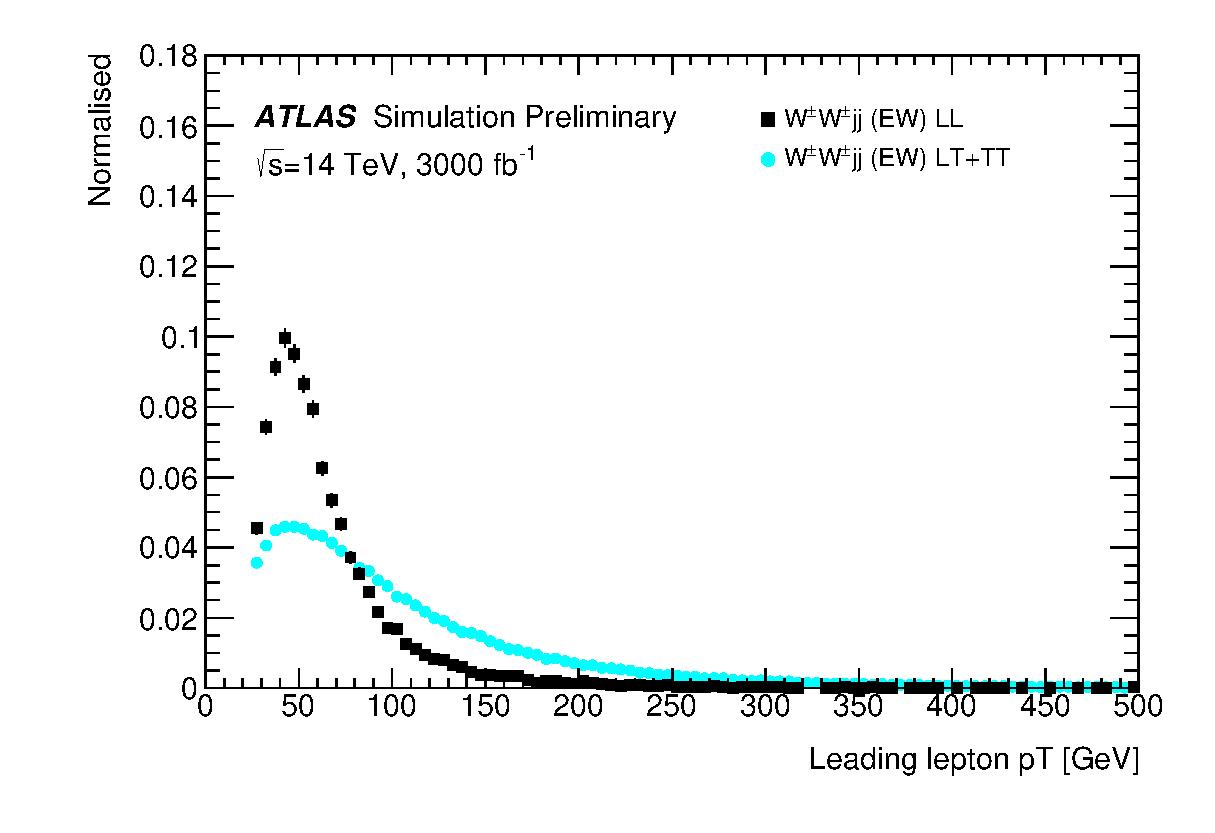
\includegraphics[width=0.48\textwidth]{figs/ssww_upgrade/polarization/lepton0_pt_pass9}
  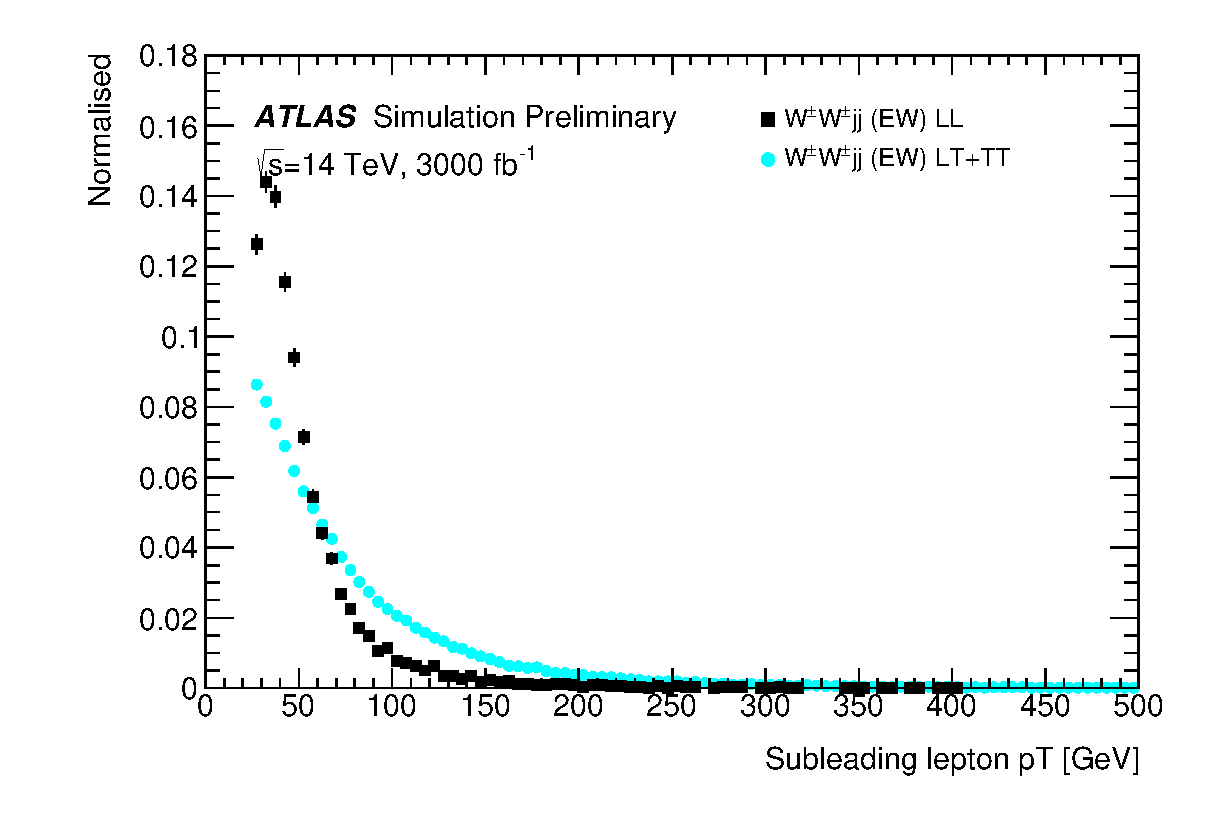
\includegraphics[width=0.48\textwidth]{figs/ssww_upgrade/polarization/lepton1_pt_pass9}
  \caption{Comparison of the leading (left) and subleading (right) lepton $\pt$ distributions for purely longitudinal (LL, black) and mixed polarization (LT+TT, cyan) \ssww events.}
  \label{fig:polarization_leppt}
\end{figure}

\begin{figure}[htp]
  \centering
  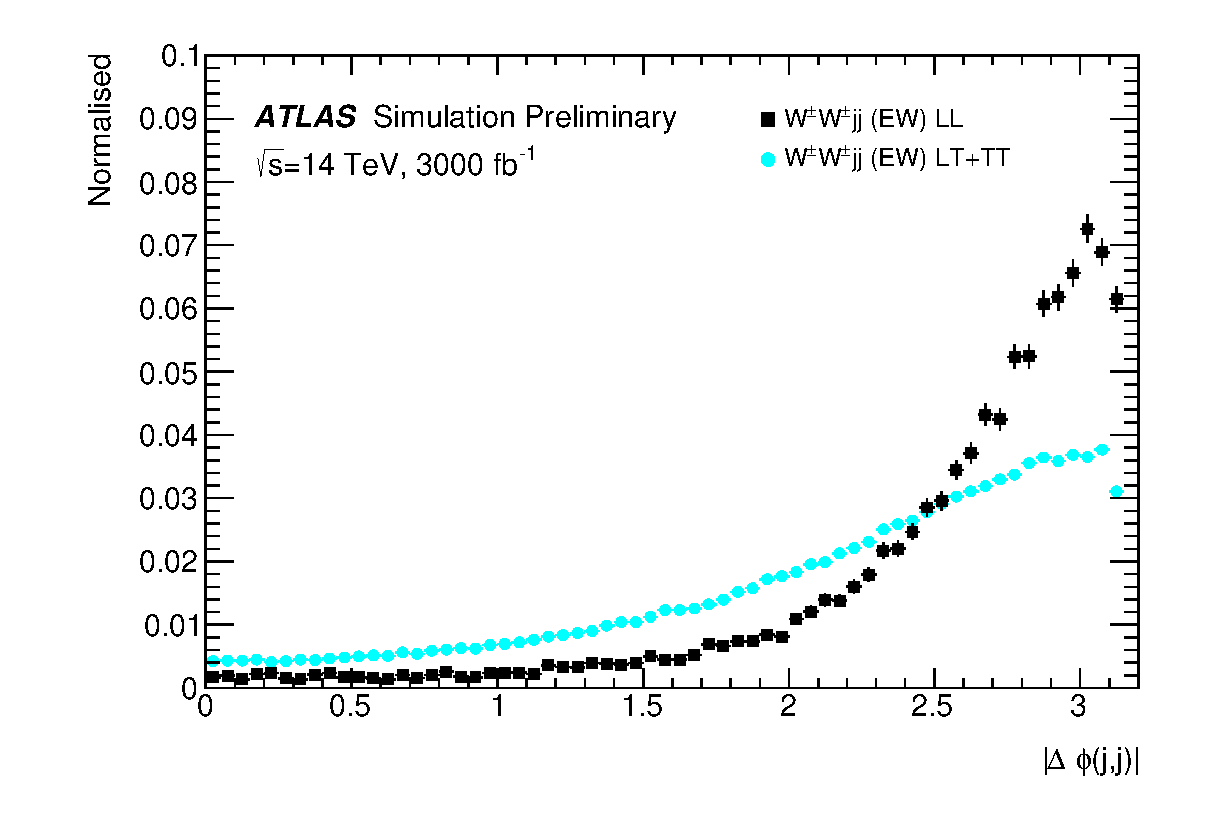
\includegraphics[width=0.48\textwidth]{figs/ssww_upgrade/polarization/dijet_absdphijj_pass9}
  \caption{Comparison of the azimuthal dijet separation ($|\dphijj|$) for purely longitudinal (LL, black) and mixed polarization (LT+TT, cyan) \ssww events.}
  \label{fig:polarization_dphijj}
\end{figure}
